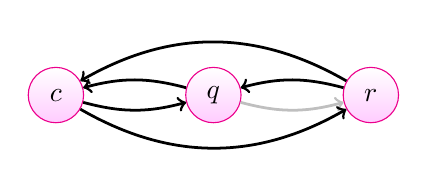
\begin{tikzpicture}

\tikzset{nodo/.style={circle,minimum size=20pt,inner sep=0pt,draw, top color=white ,bottom color=magenta!20, magenta,text=black}}
\tikzset{label/.style={minimum size=15pt,inner sep=0pt,},}





\draw (2,-3.5) node[nodo](c2) {$c$};
\draw (4,-3.5) node[nodo](q2) {$q$};
\draw (6,-3.5) node[nodo](r2) {$r$};
\draw[->,line width=1pt] (c2) to[bend right=15] (q2);
\draw[->,line width=1pt] (q2) to[bend right=15] (c2);
\draw[->,line width=1pt] (r2) to[bend right=15] (q2);
\draw[->,line width=1pt, gray!50] (q2) to[bend right=15] (r2);
\draw[->,line width=1pt] (c2) to[bend right=30] (r2);
\draw[->,line width=1pt] (r2) to[bend right=30] (c2);


\end{tikzpicture}
